\documentclass{anstrans}
%%%%%%%%%%%%%%%%%%%%%%%%%%%%%%%%%%%
\title{Benefits of Siting a Borehole Repository at a Non-operating Nuclear 
Facility}
\author{Jin Whan Bae,$^{*}$ Abraham Lincoln$^{\dagger}$}

\institute{
$^{*}$Dept. of Nuclear Plasma, and Radiological Engineering, University of Illinois at Urbana-Champaign, Urbana, IL
\and
$^{\dagger}$State Capitol Building, Springfield, IL
}

\email{jbae11@illinois.edu \and honestabe@example.com}

%%%% packages and definitions (optional)
\usepackage{graphicx} % allows inclusion of graphics
\usepackage{booktabs} % nice rules (thick lines) for tables
\usepackage{microtype} % improves typography for PDF

\newcommand{\SN}{S$_N$}
\renewcommand{\vec}[1]{\bm{#1}} %vector is bold italic
\newcommand{\vd}{\bm{\cdot}} % slightly bold vector dot
\newcommand{\grad}{\vec{\nabla}} % gradient
\newcommand{\ud}{\mathop{}\!\mathrm{d}} % upright derivative symbol

\begin{document}
%%%%%%%%%%%%%%%%%%%%%%%%%%%%%%%%%%%%%%%%%%%%%%%%%%%%%%%%%%%%%%%%%%%%%%%%%%%%%%%%
\section{Introduction}

Introduction material here. To cite something, use bibtex \cite{Lar2008} and 
don't forget to put the citation in the bib file. Use the ARFC group Zotero 
folder to compile references. 


%%%%%%%%%%%%%%%%%%%%%%%%%%%%%%%%%%%%%%%%%%%%%%%%%%%%%%%%%%%%%%%%%%%%%%%%%%%%%%%%

\subsection{Background}
What do people need to know about past work to read this paper.

\subsection{Motivation}
Here's where we put the motivation.


%%%%%%%%%%%%%%%%%%%%%%%%%%%%%%%%%%%%%%%%%%%%%%%%%%%%%%%%%%%%%%%%%%%%%%%%%%%%%%%%
\section{Results and Analysis}
The results were interesting, so interesting in fact that we have decided to
present them here.

Figure~\ref{fig:voltage} shows how a plot might conceivably look in your
document. Always place figures after they are referenced so as not to throw
off the reader. You can use symbols and different line styles to help
differentiate your results, especially if they are printed in black and white.
Note how Fig.~\ref{fig:voltage} uses dashed lines \verb|--| for the exact
solution, solid lines \verb|-| for the new method's solutions, and dotted lines
\verb|:| for existing inaccurate methods.
\begin{figure}[ht] % replace 't' with 'b' to force it to be on the bottom
  \centering
  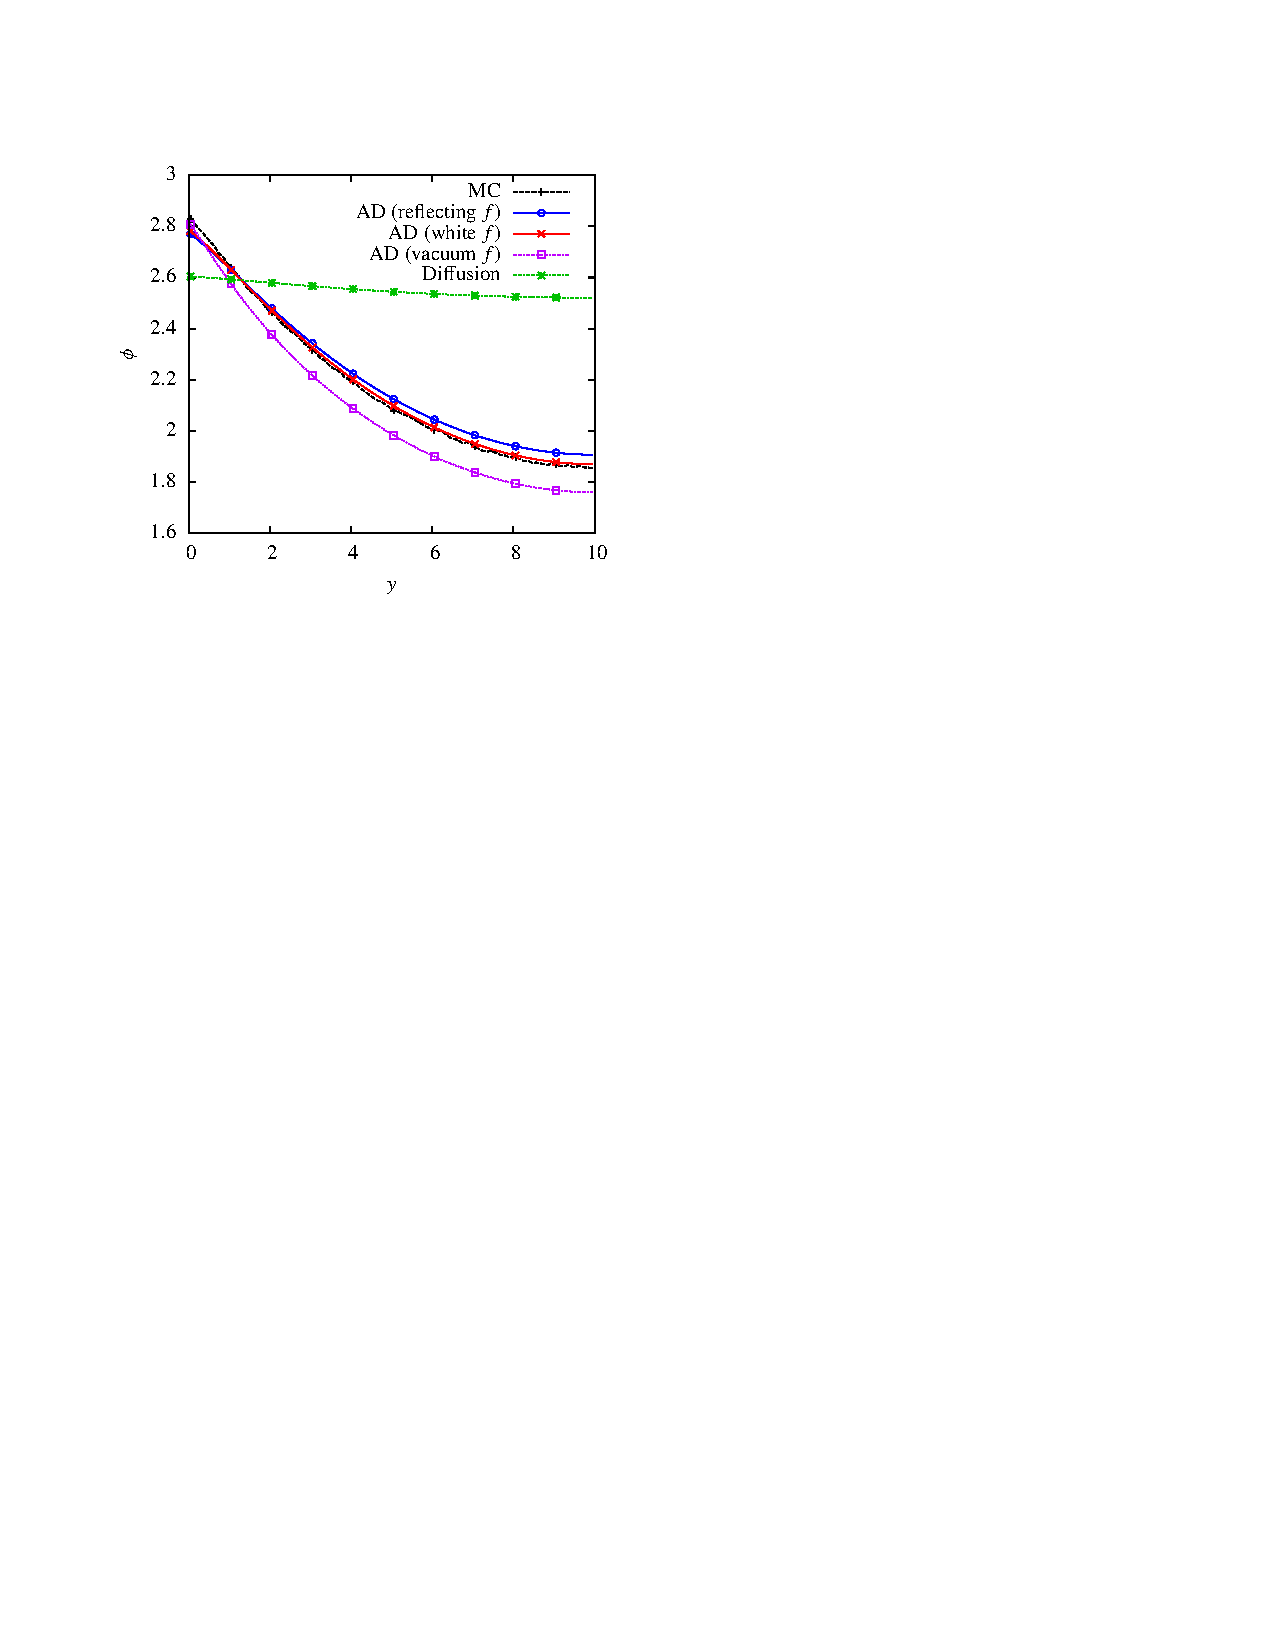
\includegraphics{example_figure}
  \caption{Captions are flush with the left.}
  \label{fig:voltage}
\end{figure}

Later on, we can include a table, even one that spans two columns such as
Table~\ref{tab:widetable}.
%%%%%%%%%%%%%%%%%%%%%%%%%%%%%%%%%%%%%%%%
\begin{table*}[htb]
  \centering
\begin{tabular}{llllllllll}\toprule
      & $\phi_T(0)$      & $\phi_T(10)$      & $\phi_T(20)$      &
      $\phi_D(0)$      & $\phi_D(10)$      & $\phi_D(20)$      & $\rho$      &
      $\varepsilon$      & $N_\text{it}$
\\ \midrule
$c=0.999$  & 0.9038 & 20.63 & 31.24 & 0.9087 & 20.63 & 31.23 & 0.2192 & $10^{-7}$ & 15
\\
$c=0.990$  & 0.3675 & 13.04 & 24.7 & 0.3696 & 13.04 & 24.69 & 0.2184 & $10^{-7}$ & 15
\\
$c=0.900$  & 0.009909 & 4.776 & 17.64 & 0.009984 & 4.786 & 17.63 & 0.2118 & $10^{-7}$ & 14
\\
$c=0.500$  & $6.069\times 10^{-5}$ & 2.212 & 15.53 & 6.213$\times 10^{-5}$ & 2.239 & 15.53 & 0.2068 & $10^{-7}$ & 13
\\
\bottomrule
\end{tabular}
  \caption{This is an example of a really wide table which might not normally
  fit in the document.}
  \label{tab:widetable}
\end{table*}
%%%%%%%%%%%%%%%%%%%%%%%%%%%%%%%%%%%%%%%%
Notice how the table reference uses a Roman numeral
for its numbering scheme, whereas the figure reference uses an Arabic numeral.
For one-column tables, use the \verb|table| environment; two-column tables use
\verb|table*|. The same applies to figures.

%%%%%%%%%%%%%%%%%%%%%%%%%%%%%%%%%%%%%%%%%%%%%%%%%%%%%%%%%%%%%%%%%%%%%%%%%%%%%%%%
\section{Conclusions}

Put your conclusions here. 

%%%%%%%%%%%%%%%%%%%%%%%%%%%%%%%%%%%%%%%%%%%%%%%%%%%%%%%%%%%%%%%%%%%%%%%%%%%%%%%%
\section{Acknowledgments}

This material is based upon work supported by ACDIS.

%%%%%%%%%%%%%%%%%%%%%%%%%%%%%%%%%%%%%%%%%%%%%%%%%%%%%%%%%%%%%%%%%%%%%%%%%%%%%%%%
\bibliographystyle{ans}
\bibliography{bibliography}
\end{document}
